\chapter {IMPLEMENTASI}
\par Bab ini membahas implementasi dari rancangan sistem yang ada pada bab 3. Bahasa pemrograman yang digunakan untuk implementasi aplikasi \textit{push notification}.

\section{Lingkungan Implementasi}
\par Lingkungan implementasi yang digunakan untuk mengembangkan tugas akhir ini memiliki spesifikasi perangkat keras dan lunak seperti ditampilkan pada tabel~\ref{tabel_spesifikasi_server}, tabel~\ref{tabel_spesifikasi_perangkat_android}, dan tabel~\ref{tabel_spesifikasi_perangkat_ios}.
\begin{longtable}{|p{2.5cm}|p{6.5cm}|}
    \hline
    \textbf{Jenis} & \textbf{Spesifikasi} \\ \hline
    CPU & AMD Ryzen 5 2500U \\ \hline
    CPU Core & 4 \\ \hline
    Memory & 12 GB \\ \hline
    Sistem Operasi & Ubuntu 19.04 \\ \hline
    Kakas Bantu &
    \begin{enumerate}
        \item Intellij IDEA
        \item DataGrip
    \end{enumerate} \\ \hline
    \caption{Spesifikasi Server}
    \label{tabel_spesifikasi_server}
\end{longtable}
\begin{longtable}{|p{2.5cm}|p{6.5cm}|}
    \hline
    \textbf{Jenis} & \textbf{Spesifikasi} \\ \hline
    CPU & Snapdragon 636 \\ \hline
    Memory & 3 GB \\ \hline
    Sistem Operasi & Android 9 (Pie) \\ \hline
    \caption{Spesifikasi Perangkat Android}
    \label{tabel_spesifikasi_perangkat_android}
\end{longtable}
\begin{longtable}{|p{2.5cm}|p{6.5cm}|}
    \hline
    \textbf{Jenis} & \textbf{Spesifikasi} \\ \hline
    CPU & Apple A10 Fusion \\ \hline
    Memory & 3 GB \\ \hline
    Sistem Operasi & iOS 12 \\ \hline
    \caption{Spesifikasi Perangkat iOS}
    \label{tabel_spesifikasi_perangkat_ios}
\end{longtable}

\section{Implementasi Basis Data}
\par Subbab ini membahas struktur tabel yang digunakan, meliputi tujuan pembuatan tabel, Kode yang digunakan untuk membuat tabel, dan gambar tabel yang telah dibuat.

\subsection{Implementasi Tabel User}
\par Tabel ini digunakan untuk menyimpan data pengguna. Kode yang digunakan untuk membuat tabel dapat dilihat pada kode sumber~\ref{code:user_account}, dan hasil tabel dapat dilihat pada gambar~\ref{tabel_user_account}.
\lstinputlisting[label=code:user_account, caption=Implementasi Tabel User, language=SQL]{bab4/codes/user_account.sql}
\begin{figure}[H]
    \centering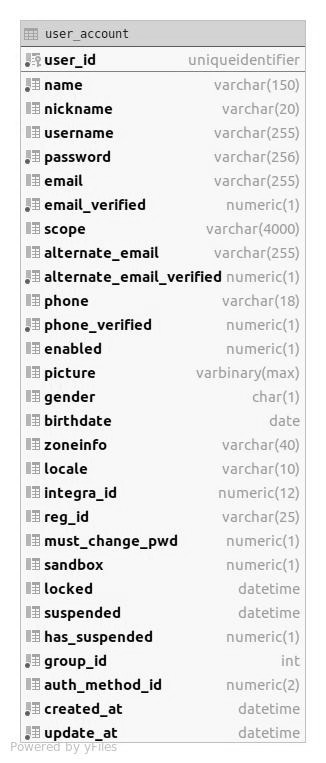
\includegraphics[width=0.5\textwidth]{bab4/figures/tabel_user_account.jpg}
    \caption{Tabel User (user\_account)}
    \label{tabel_user_account}
\end{figure}

\subsection{Implementasi Tabel Group}
\par Tabel ini digunakan untuk menyimpan data kelompok pengguna. Kode yang digunakan untuk membuat tabel dapat dilihat pada kode sumber~\ref{code:pn_group}, dan hasil tabel dapat dilihat pada gambar~\ref{tabel_pn_group}.
\lstinputlisting[label=code:pn_group, caption=Implementasi Tabel Group, language=SQL]{bab4/codes/pn_group.sql}
\begin{figure}[H]
    \centering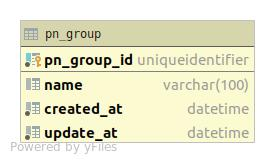
\includegraphics[width=0.5\textwidth]{bab4/figures/tabel_pn_group.jpg}
    \caption{Tabel Group (pn\_group)}
    \label{tabel_pn_group}
\end{figure}

\subsection{Implementasi Tabel Group Member}
\par Tabel ini digunakan untuk menyimpan data anggota kelompok pengguna. Kode yang digunakan untuk membuat tabel dapat dilihat pada kode sumber~\ref{code:pn_group_member}, dan hasil tabel dapat dilihat pada gambar~\ref{tabel_pn_group_member}.
\lstinputlisting[label=code:pn_group_member, caption=Implementasi Tabel Group Member, language=SQL]{bab4/codes/pn_group_member.sql}
\begin{figure}[H]
    \centering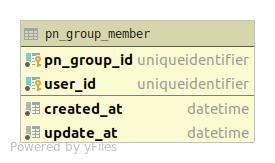
\includegraphics[width=0.5\textwidth]{bab4/figures/tabel_pn_group_member.jpg}
    \caption{Tabel Group Member (pn\_group\_member)}
    \label{tabel_pn_group_member}
\end{figure}

\subsection{Implementasi Tabel Client}
\par Tabel ini digunakan untuk menyimpan data client (aplikasi). Kode yang digunakan untuk membuat tabel dapat dilihat pada kode sumber~\ref{code:oauth_client}, dan hasil tabel dapat dilihat pada gambar~\ref{tabel_oauth_client}.
\lstinputlisting[label=code:oauth_client, caption=Implementasi Tabel Client, language=SQL]{bab4/codes/oauth_client.sql}
\begin{figure}[H]
    \centering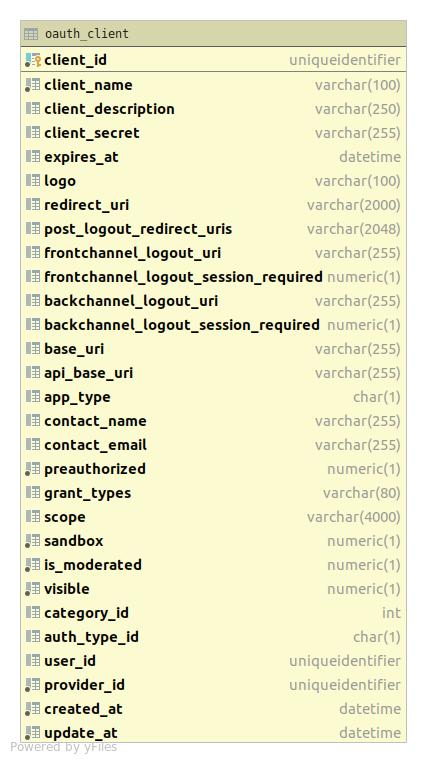
\includegraphics[width=0.5\textwidth]{bab4/figures/tabel_oauth_client.jpg}
    \caption{Tabel Client (oauth\_client)}
    \label{tabel_oauth_client}
\end{figure}

\subsection{Implementasi Tabel Certificate}
\par Tabel ini digunakan untuk menyimpan data sertifikat client untuk autentikasi ke layanan APNs dan FCM. Kode yang digunakan untuk membuat tabel dapat dilihat pada kode sumber~\ref{code:pn_certificate}, dan hasil tabel dapat dilihat pada gambar~\ref{tabel_pn_certificate}.
\lstinputlisting[label=code:pn_certificate, caption=Implementasi Tabel Certificate, language=SQL]{bab4/codes/pn_certificate.sql}
\begin{figure}[H]
    \centering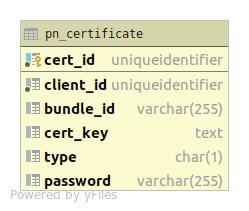
\includegraphics[width=0.5\textwidth]{bab4/figures/tabel_pn_certificate.jpg}
    \caption{Tabel Certificate (pn\_certificate)}
    \label{tabel_pn_certificate}
\end{figure}

\subsection{Implementasi Tabel Device}
\par Tabel ini digunakan untuk menyimpan data perangkat pengguna yang terdaftar di layanan APNs dan FCM. Kode yang digunakan untuk membuat tabel dapat dilihat pada kode sumber~\ref{code:device_token}, dan hasil tabel dapat dilihat pada gambar~\ref{tabel_device_token}.
\lstinputlisting[label=code:device_token, caption=Implementasi Tabel Device, language=SQL]{bab4/codes/device_token.sql}
\begin{figure}[H]
    \centering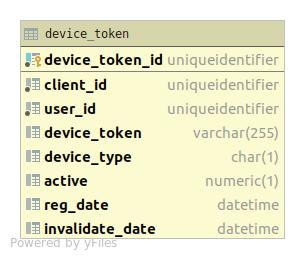
\includegraphics[width=0.5\textwidth]{bab4/figures/tabel_device_token.jpg}
    \caption{Tabel Device (device\_token)}
    \label{tabel_device_token}
\end{figure}

\subsection{Implementasi Tabel Batch}
\par Tabel ini digunakan untuk menyimpan data notifikasi yang akan dikirim ke beberapa pengguna atau kelompok. Kode yang digunakan untuk membuat tabel dapat dilihat pada kode sumber~\ref{code:pn_batch}, dan hasil tabel dapat dilihat pada gambar~\ref{tabel_pn_batch}.
\lstinputlisting[label=code:pn_batch, caption=Implementasi Tabel Batch, language=SQL]{bab4/codes/pn_batch.sql}
\begin{figure}[H]
    \centering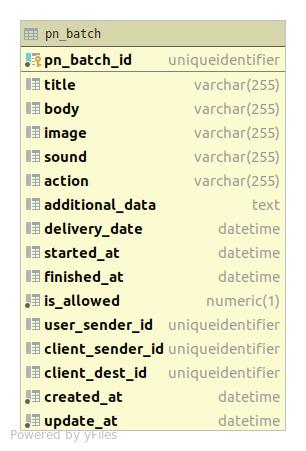
\includegraphics[width=0.5\textwidth]{bab4/figures/tabel_pn_batch.jpg}
    \caption{Tabel Batch (pn\_batch)}
    \label{tabel_pn_batch}
\end{figure}

\subsection{Implementasi Tabel Packet}
\par Tabel ini digunakan untuk menyimpan data notifikasi yang akan dikirim ke satu perangkat. Kode yang digunakan untuk membuat tabel dapat dilihat pada kode sumber~\ref{code:pn_packet}, dan hasil tabel dapat dilihat pada gambar~\ref{tabel_pn_packet}.
\lstinputlisting[label=code:pn_packet, caption=Implementasi Tabel Packet, language=SQL]{bab4/codes/pn_packet.sql}
\begin{figure}[H]
    \centering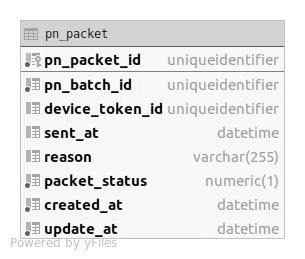
\includegraphics[width=0.5\textwidth]{bab4/figures/tabel_pn_packet.jpg}
    \caption{Tabel Packet (pn\_packet)}
    \label{tabel_pn_packet}
\end{figure}

\subsection{Implementasi Tabel User Destination}
\par Tabel ini digunakan untuk menyimpan data pengguna yang akan menerima notifikasi dari suatu batch. Kode yang digunakan untuk membuat tabel dapat dilihat pada kode sumber~\ref{code:pn_user_destination}, dan hasil tabel dapat dilihat pada gambar~\ref{tabel_pn_user_destination}.
\lstinputlisting[label=code:pn_user_destination, caption=Implementasi Tabel User Destination, language=SQL]{bab4/codes/pn_user_destination.sql}
\begin{figure}[H]
    \centering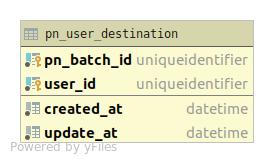
\includegraphics[width=0.5\textwidth]{bab4/figures/tabel_pn_user_destination.jpg}
    \caption{Tabel User Destination (pn\_user\_destination)}
    \label{tabel_pn_user_destination}
\end{figure}

\subsection{Implementasi Tabel Group Destination}
\par Tabel ini digunakan untuk menyimpan data kelompok yang akan menerima notifikasi dari suatu batch. Kode yang digunakan untuk membuat tabel dapat dilihat pada kode sumber~\ref{code:pn_group_destination}, dan hasil tabel dapat dilihat pada gambar~\ref{tabel_pn_group_destination}.
\lstinputlisting[label=code:pn_group_destination, caption=Implementasi Tabel Group Destination, language=SQL]{bab4/codes/pn_group_destination.sql}
\begin{figure}[H]
    \centering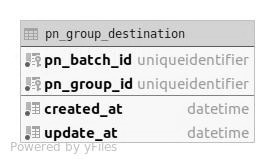
\includegraphics[width=0.5\textwidth]{bab4/figures/tabel_pn_group_destination.jpg}
    \caption{Tabel Group Destination (pn\_group\_destination)}
    \label{tabel_pn_group_destination}
\end{figure}

%TODO kopas kodingan
\section{Implementasi Proses dan Kasus Penggunaan}
\par Subbab ini membahas implementasi proses yang dibuat berdasarkan hasil analisa dan rancangan yang telah dilakukan.

\subsection{Implementasi Pembuatan Packet}
\par Proses pembuatan packet dilakukan secara berkala oleh modul Scheduler dengan jeda waktu 30 detik. Proses ini diawali dengan mencari batch-batch yang belum dan boleh dibuatkan packet dari sistem basis data, lalu untuk setiap batch akan diolah menjadi packet-packet dan disimpan ke sistem basis data. Proses pembuatan packet dilakukan dengan mencari data device yang menjadi penerima notifikasi dari sebuah batch, lalu untuk setiap device akan diolah menjadi packet. Setelah proses pembuatan packet selesai, data waktu mulai dan selesai batch akan diperbarui berdasarkan waktu awal dan akhir pembuatan packet. Potongan kode yang digunakan untuk pembuatan packet dapat dilihat pada kode sumber~X.

\subsubsection{Implementasi Menambahkan Packet ke Antrian}
\par Proses penambahan packet ke antrian dilakukan secara berkala oleh modul Scheduler dengan jeda waktu 30 detik dan jeda awal 15 detik. Penambahan jeda awal ini bertujuan agar pembuatan dan pengantrian packet tidak berjalan secara bersamaan, sehingga dapat mengurangi beban pada sistem basis data. Proses ini diawali dengan mencari packet yang belum dan sudah waktunya dikirim dari sistem basis data. Packet-packet tersebut akan diperbarui statusnya menjadi menunggu, dan dikirim ke antrian, dengan pembagian topik sesuai dengan jenis device penerima notifikasi. Potongan kode yang digunakan untuk menambahkan packet ke antrian dapat dilihat pada kode sumber~X.

\subsection{Implementasi Pengiriman Packet ke APNs}
\par Proses pengiriman packet dilakukan secara berkala oleh Sender APN dengan cara menunggu Kafka untuk mengirimkan data packet yang berada diantrian. Proses ini diawali dengan Sender APN mendaftarkan diri di Kafka sebagai consumer untuk topik "ios". Setelah Sender APN terdaftar, Kafka akan mengirimkan packet yang ada di antrian topik "ios" secara berkala ke Sender APN. Setelah packet diterima, Sender APN akan mengirimkan request notifikasi berdasarkan data packet ke layanan APNs. Setelah request berhasil, status packet akan diperbarui sesuai dengan response dari layanan APNs. Potongan kode yang digunakan untuk pengiriman packet ke APNs dapat dilihat pada kode sumber~X.

\subsection{Implementasi Pengiriman Packet ke FCM}
\par Proses pengiriman packet dilakukan secara berkala oleh Sender FCM dengan cara menunggu Kafka untuk mengirimkan data packet yang berada diantrian. Proses ini diawali dengan Sender FCM mendaftarkan diri di Kafka sebagai consumer untuk topik "android" dan "web". Setelah Sender FCM terdaftar, Kafka akan mengirimkan packet yang ada di antrian topik "android" dan "web" secara berkala ke Sender FCM. Setelah packet diterima, Sender FCM akan mengirimkan request notifikasi berdasarkan data packet ke layanan FCM. Setelah request berhasil, status packet akan diperbarui sesuai dengan response dari layanan FCM. Potongan kode yang digunakan untuk pengiriman packet ke FCM dapat dilihat pada kode sumber~X.

\subsection{Implementasi Pemantauan Aplikasi}
\par Proses pemantauan aplikasi (menampilkan penggunaan sumber daya, menampilkan status kesehatan, menampilkan konfigurasi, menampilkan log) diimplementasikan dengan menggunakan library Spring Boot Actuator dan Spring Boot Admin. Spring Boot Actuator digunakan untuk menampilkan hasil pemantauan dalam bentuk REST API, sementara Spring Boot Admin digunakan untuk menampilkan hasil pemantauan yang dilakukan oleh Spring Boot Actuator dalam bentuk halaman web. Potongan kode yang digunakan untuk konfigurasi Spring Boot Actuator dan Spring Boot Admin dapat dilihat pada kode sumber~X.
